\documentclass[../main.tex]{subfiles}

\begin{document}

\section{Determinants}

Finally determinants! One of the most foundational concepts in linear
algebra is the determinant. Being one of the foundational concepts,
I also think it is a hard concept if the intuition is excluded in the
discussion due to its formula heavy nature.

As you could have noticed, a linear transformation does not only
change the position of the vectors. Consider the following diagram.

\begin{figure}[H]
\centering
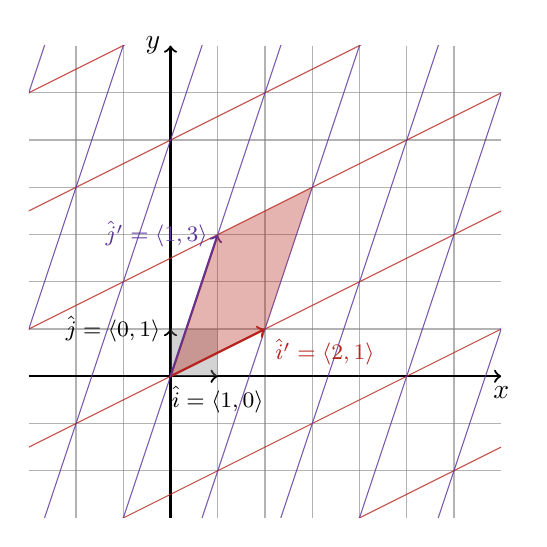
\begin{tikzpicture}[
        vector/.style={->, thick},
        scale=0.6
    ]

    \foreach \i in {-2, -1, ..., 6} {
        \draw[gray, thin, opacity=0.6] (\i, -3) -- (\i, 7);
        \draw[gray, thin, opacity=0.6] (-3, \i) -- (7, \i);
    }
    \draw[vector, black] (-3, 0) -- (7, 0) node[below] {$x$};
    \draw[vector, black] (0, -3) -- (0, 7) node[left] {$y$};

    \draw[vector] (0, 0) -- (1, 0) node[below]
        {\footnotesize $\hat{i} = \langle 1, 0 \rangle$};
    \draw[vector] (0, 0) -- (0, 1) node[left]
        {\footnotesize $\hat{j} = \langle 0, 1 \rangle$};
    \fill[Gray, opacity=0.35]
        (0,0) -- (1,0) -- (1,1) -- (0,1) -- cycle;

    \begin{scope}
        \clip (-3, -3) rectangle (7, 7);

        \foreach \j in {-10, -9, ..., 10} {
            \draw[BrickRed, opacity=0.8]
                ({-10*2 + \j*1}, {-10*1 + \j*3})
                    -- ({10*2 + \j*1}, {10*1 + \j*3});
        }
        \foreach \i in {-10, -9, ..., 10} {
            \draw[RoyalPurple, opacity=0.8]
                ({\i*2 + -10*1}, {\i*1 + -10*3})
                    -- ({\i*2 + 10*1}, {\i*1 + 10*3});
        }
    \end{scope}

    \draw[vector, BrickRed] (0, 0) -- (2, 1)
        node[below right, BrickRed]
            {\footnotesize $\hat{i}' = \langle 2, 1 \rangle$};
    \draw[vector, RoyalPurple] (0, 0) -- (1, 3)
        node[left, RoyalPurple]
            {\footnotesize $\hat{j}' = \langle 1, 3 \rangle$};
    \fill[BrickRed, opacity=0.35]
        (0,0) -- (2,1) -- (3,4) -- (1,3) -- cycle;
\end{tikzpicture}
\end{figure}

Notice that from the diagram above, the gray area is scaled to the
new red area. Notice that the area of the new parallelogram is
$3 \cdot 4 - 1 \cdot 2 \cdot \frac{1}{2} \cdot 2 - 1 \cdot 3 \cdot
\frac{1}{2} \cdot 2 - 1 \cdot 2 = 12 - 2 - 3 - 2 = 5$. Because
the area which was originally $1$ is scaled to $5$, we can say that
\[
\begin{vmatrix}
    2 & 1 \\
    1 & 3
\end{vmatrix}
= 5
\]
holds. The determinant is only defined for square matrices, and for
each square matrix, the determinants tell how much the area has
changed after the linear transformation. Determinants can surely
be negative, and they represent the change in orientation.
With this intuition in mind, let's discuss more computational
perspective of determinants.

Before we discuss the formula for determinants, let's define a
notation.

\begin{definition}{}{}
The \textbf{minor} of matrix $A$, denoted as $M_{ij}$, is a submatrix
of $A$ without the $i^\text{th}$ row and $j^\text{th}$ column of $A$.
The \textbf{cofactor} of $a_{ij}$ is defined as $(-1)^{i+j}
\det(M_{ij})$.
\end{definition}

Consider the following examples for $A$ defined as the following.
\[
A =
\begin{bmatrix}
    a_{11} & a_{12} & a_{13} & a_{14} \\
    a_{21} & a_{22} & a_{23} & a_{24} \\
    a_{31} & a_{32} & a_{33} & a_{34} \\
    a_{41} & a_{42} & a_{43} & a_{44}
\end{bmatrix}
\]
$M_{11}$ and $M_{24}$ are defined as the following.
\[
M_{11} =
\begin{bmatrix}
    a_{22} & a_{23} & a_{24} \\
    a_{32} & a_{33} & a_{34} \\
    a_{42} & a_{43} & a_{44}
\end{bmatrix}, \quad
M_{24} =
\begin{bmatrix}
    a_{11} & a_{12} & a_{13} \\
    a_{31} & a_{32} & a_{33} \\
    a_{41} & a_{42} & a_{43}
\end{bmatrix}
\]
Now let's define what determinants are with a recursive formula.

\begin{definition}{}{}
The \textbf{determinant} of a square matrix $A$, denoted as $\det(A)$
or $|A|$, is a value defined with the following rules.
\begin{enumerate}[noitemsep]
\item $\det(A) = a_{11}$ if $A = [a_{11}]$.
\item The following equation can be used to determine $\det(A)$ for
$A$ with order $n \times n$ for $n > 1$.
\[
\det(A)
= \sum_{j=1}^n (-1)^{1 + j} a_{1j} \det(M_{1j})
\]
\end{enumerate}
\end{definition}

Let's take a look at an example with a $2 \times 2$ matrix
$A = [a_{ij}]$.
\begin{align*}
    \det(A)
    &= \sum_{j=1}^2 (-1)^{1 + j} a_{1j} \det(M_{1j})
    = (-1)^{1 + 1} a_{11} \det(M_{11}) +
        (-1)^{1 + 2} a_{12} \det(M_{12}) \\
    &= (-1)^{2} a_{11} a_{22} + (-1)^{3} a_{12} a_{21} \\
    &= a_{11} a_{22} - a_{12} a_{21}
\end{align*}
Returning to our first example, we can verify that the formula holds.
\[
\begin{vmatrix}
    2 & 1 \\
    1 & 3
\end{vmatrix}
= 2 \cdot 3 - 1 \cdot 1
= 5
\]
We could also derive the formula for higher orders with many
computations but I will leave them for you! I also think it is
just better to use the recursive formula and the formula for
$2 \times 2$ matrices instead of memorizing complex formulas,
but I don't know. I think it's up to you. Below is another
example.
\[
\det\left(
    \begin{bmatrix}
        1 & 0 & 0 \\
        0 & 1 & 0 \\
        0 & 0 & 1
    \end{bmatrix}
\right)
= \sum_{j=1}^3 (-1)^{1 + j} a_{1j} \det(M_{1j})
= a_{11} \det(M_{11})
= 1 \cdot 1 - 0 \cdot 0 = 1
\]
With these in mind, we can establish a very important theorem in
computing determinants.

\begin{theorem}{}{Cofactor Expansion}
For any square matrix $A$, the cofactor expansion along the
$i^\text{th}$ row and the cofactor expansion along the $j^\text{th}$
column equal. In other words, the following equation holds.
\[
\det(A)
= \sum_{j=1}^n (-1)^{i + j} a_{ij} \det(M_{ij})
= \sum_{i=1}^n (-1)^{i + j} a_{ij} \det(M_{ij})
\]
\end{theorem}

Let's save the proof for the theorem for later as we need to show
different properties of determinants before proving the theorem
above. For now, let's discuss a special property of triangular
matrices.

\begin{theorem}{}{The Determinants of Triangular Matrices}
For a triangular (upper or lower) matrix $A_{n \times n} = [a_{ij}]$,
the determinant is defined as the following.
\[
\det(A)
= \prod_{i=1}^n a_{ii}
\]
\end{theorem}
\begin{proof}
First, the case for upper triangular matrix can be proven. Notice that
\[
\det(A)
= \sum_{i=1}^n (-1)^{i + 1} a_{i1} \det(M_{i1})
= a_{11} \det(M_{11})
\]
by Theorem \ref{theo:Cofactor Expansion}. Continuing, notice that
$M_{11}$ is another upper triangular matrix by definition.

If such calculations are continued, it is evident that the last
term would be $a_{nn}$. Similarly, the second to the last term
would be $a_{nn} a_{n-1,n-1}$. By inductive hypothesis, it is
evident that
\[
\det(A)
= a_{11} \det(M_{11})
= a_{11} \prod_{i=2}^n a_{ii}
= \prod_{i=1}^n a_{ii}
\]
and the theorem holds for upper triangular matrix.

The case for lower triangular matrix can be proven in similar
manner. Note that $\det(A) = \sum_{j=1}^n (-1)^{1 + j} a_{1j}
\det(M_{1j}) = a_{11} \det(M_{11})$. With the same inductive
hypothesis above, it can be concluded that
\[
\det(A)
= a_{11} \det(M_{11})
= a_{11} \prod_{i=2}^n a_{ii}
= \prod_{i=1}^n a_{ii}
\]
and the theorem holds.
\end{proof}

As you could have guessed, we get a direct corollary from the
theorem.

\begin{corollary}{}{Determinants of Diagonal Matrices}
The determinant of any diagonal matrix is the product of the
diagonal entries.
\end{corollary}
\begin{proof}
First and foremost, notice that a diagonal matrix is both
an upper and lower triangular matrix. Thus by Theorem \ref{theo:The
Determinants of Triangular Matrices}, the corollary holds.
\end{proof}

Continuing from triangular matrices, we can also apply our
understanding of a transpose of a matrix. Consider the following
theorem.

\begin{theorem}{}{Transpose and Determinants}
$\det(A) = \det(A^\intercal)$ holds for all square matrix $A$.
\end{theorem}
\begin{proof}
First and foremost, notice that $A = A^\intercal$ if $A$ is a
$1 \times 1$ matrix. Thus, the theorem holds for any $A_{1 \times 1}$.
Continuing, note that for $A_{n \times n}$ with $n > 1$, $M_{ij}$
equals $M'_{ij}$ for $A^T$. Moreover by definition, $M'_{ij} =
M_{ji}$ and the following equation holds $A^\intercal = [a'_{ij}]$.
\[
\det(A)
= \sum_{i=1}^n (-1)^{i + 1} a_{i1} \det(M_{i1})
= \sum_{j=1}^n (-1)^{1 + j} a'_{1j} \det(M'_{1j})
= \det\left( A^\intercal \right)
\]
Thus, the theorem holds.
\end{proof}

Now that we discussed the relationships between matrices and
determinants, let's conclude our discussion with products and
determinants.

\subsection{Determinant and Products}

Before we conclude our discussion on determinant and this note,
I wished to introduce one of the most important results of
determinants. In this part of the section, we will try to prove
that the product of the determinants is the same as the determinant
of the product. To prove this result, we would need a lot of lemmas,
so let's get started with the first one.

\begin{lemma}{}{Determinants and Elementary Matrices I}
For a matrix $A_{n \times n}$ and an elementary matrix
$E_{n \times n}$ for interchanging two rows, $\det(E) = -1$
and $\det(EA) = \det(E) \det(A)$.
\end{lemma}
\begin{proof}
First and foremost, the case when $E$ exchanges two consecutive
rows can be proven. Let $B = FA$ where $F$ is the $n \times n$
elementary matrix that interchanges the $k^\text{th}$ and
$k+1^\text{th}$ rows of $A$. Therefore, for $A = [a_{ij}]$ and
$B = [b_{ij}]$, $b_{k+1,j} = a_{kj}$ holds and for the minor of $B$ as
$M'_{ij}$, $M'_{i+1,j} = M_{ij}$. Moreover, notice that $F = -1$ for
$n = 2$ and by inductive hypothesis with exchanging the use of
$\det(A) = (-1)^2 a_{11} \det(M_{11})$ and $\det(A) = (-1)^{2n} a_{nn}
\det(M_{nn})$, it is evident that $\det(F) = -1$. Thus, the following
equations hold.
\begin{align*}
    \det(B)
    &= \sum_{j=1}^n (-1)^{k+1+j} b_{k+1,j} \det(M'_{k+1,j}) \\
    &= \sum_{j=1}^n (-1)^{k+1+j} a_{kj} \det(M_{kj})
    = -\sum_{j=1}^n (-1)^{k+j} a_{kj} \det(M_{kj}) \\
    &= -\det(A)
\end{align*}
Thus, $\det(FA) = \det(F) \cdot \det(A)$. Continuing, notice that
any exchange between two consecutive rows requires one $F$. Moreover,
any exchange between two rows with a row in between requires three
$F$s. Since any exchange can be performed with the combination of
such two operations, it is evident that every $E$ can be represented
as odd number of $F$s. Therefore, the following equations hold for
odd $m$.
\begin{align*}
    \det(EA)
    &= \det(F_1 F_2 \cdots F_m A)
    = \det(F_1) \det(F_2) \cdots \det(F_m) \det(A) \\
    &= (-1)^m \det(A)
    = -\det(A) \\
    &= \det(E) \det(A)
\end{align*}
Thus, the lemma holds.
\end{proof}

Continuing from this lemma, we can establish an interesting corollary.

\begin{corollary}{}{Identical Rows or Columns and Determinant}
The equation $\det(A) = 0$ holds for all square matrices $A$ with
either two identical rows or columns.
\end{corollary}
\begin{proof}
Let $k_1$ and $k_2$ be the identical rows of the matrix $A$.
For an elementary matrix $E$ that interchanges the rows $k_1$ and
$k_2$, the following equations hold by Lemma \ref{lem:Determinants
and Elementary Matrices I}.
\[
\det(A)
= \det(EA)
= \det(E) \det(A)
= -\det(A)
\]
Thus, $\det(A) = 0$. Similarly, if $A$ has two identical columns
$k_1$ and $k_2$, the same argument applies by Theorem
\ref{theo:Transpose and Determinants} as $\det(A) =
\det(A^\intercal)$.
\end{proof}

For our second lemma, we have another elementary row operation.

\begin{lemma}{}{Determinants and Elementary Matrices II}
For a matrix $A_{n \times n}$ and an elementary matrix
$E_{n \times n}$ that scales $k^\text{th}$ row of $A$ by some nonzero
scalar $\lambda$, $\det(E) = \lambda$ and $\det(EA) = \det(E)
\det(A)$.
\end{lemma}
\begin{proof}
First because $E_{n \times n} = k$, it is evident that utilizing
$\det(A) = (-1)^2 a_{11} \det(M_{11})$ and $\det(A) = (-1)^{2n} a_{nn}
\det(M_{nn})$, appropriately will lead to $\det(E) = \lambda$ with
inductive hypothesis. Moreover, consider the following equations.
\begin{align*}
    \det(EA)
    &= \sum_{i=1}^n (-1)^{1+k} \lambda a_{ik} \det(M_{ik})
    = \lambda \sum_{i=1}^n (-1)^{1+k} a_{ik} \det(M_{ik}) \\
    &= \lambda \det(A) = \det(E) \det(A)
\end{align*}
Thus, the lemma holds.
\end{proof}

Just like our first lemma, we can expand this second lemma with
an interesting corollary.

\begin{corollary}{}{Scalars and Determinants}
For any matrix $A_{n \times n}$ and scalars $\lambda$,
$\det(\lambda A) = \lambda^n \det(A)$.
\end{corollary}
\begin{proof}
Let $E_k$ be the elementary row operation that scales the
$k^\text{th}$ row of $A$ by $\lambda$. Then, the following equations
hold by Lemma \ref{lem:Determinants and Elementary Matrices II}.
\[
\det(\lambda A)
= \det( E_n E_{n-1} \cdots E_1 A)
= \det(E_n) \det(E_{n-1}) \cdots \det(E_1) \det(A)
= \lambda^n \det(A)
\]
Thus, the corollary holds.
\end{proof}

Below is the third lemma on determinants and elementary matrices.

\begin{lemma}{}{Determinants and Elementary Matrices III}
For a matrix $A_{n \times n}$ and an elementary matrix $E$ of
the same order that adds $\lambda$ times row $k_1$ to row $k_2$
of $A$, then $\det(E) = 1$ and $\det(EA) = \det(E) \det(A)$.
\end{lemma}
\begin{proof}
First and foremost, notice that $E$ is a triangular matrix and
the elements in its diagonal are all $1$. Thus by Theorem
\ref{theo:The Determinants of Triangular Matrices}, $\det(E) = 1$.

Consider a new matrix $B$ that is obtained by replacing $k_2$
with $k_1$ from $A$. Then, $b_{k_2j} = a_{k_1j}$ and the minor
$M'_{ij}$ of $B$ satisfy $M'_{k_2j} = M_{k_2j}$. Moreover by Corollary
\ref{cor:Identical Rows or Columns and Determinant}, $\det(B) = 0$.
Therefore, the following equations hold.
\begin{align*}
    \det(EA)
    &= \sum_{j=1}^n (-1)^{k_2 + j} (a_{k_2j} + \lambda a_{k_1j})
        \det(M_{k_2j}) \\
    &= \sum_{j=1}^n (-1)^{k_2 + j} (a_{k_2j}) \det(M_{k_2j}) +
        \lambda \sum_{j=1}^n (-1)^{k_2 + j} (a_{k_1j})
            \det(M_{k_2j}) \\
    &= \det(A) + \lambda \det(B)
    = \det(A)
\end{align*}
Thus $\det(EA) = \det(A) = \det(E) \det(A)$.
\end{proof}

With the three lemmas above, we can establish an important theorem
that links the determinants of a matrix and an elementary matrix.

\begin{theorem}{}{Elementary Matrices and Determinants}
For a matrix $A_{n \times n}$ and any elementary matrix $E$ of the
same order, $\det(EA) = \det(E) \det(A)$.
\end{theorem}
\begin{proof}
By definition, there exists three different elementary matrices that
interchanges rows, scales a row, or add a scaled row to the other.
By Lemmas \ref{lem:Determinants and Elementary Matrices I},
\ref{lem:Determinants and Elementary Matrices II}, and
\ref{lem:Determinants and Elementary Matrices III}, $\det(EA) =
\det(E) \det(A)$ for all elementary matrices $E$.
\end{proof}

Now, I know it's lots of statements, but I promise we will get to
the main result. Let's take a look at one last important result to
get to our desired theorem! This theorem and its result include
the topic of invertibility, which has not been introduced yet. Please
feel free to read Section 3.3 and return or vice versa as it shouldn't
be something too hard.

\begin{theorem}{}{Invertibility and the Determinant}
A square matrix $A$ is invertible if and only if $\det(A) \neq 0$.
\end{theorem}
\begin{proof}
First, notice that $A$ is invertible if and only if there exists a
sequence of elementary matrices $E_1, \ldots, E_k$ such that
$E_k \cdots E_1 A = U$ holds for some upper triangular matrix $A$.
In other words,
\[
\det(E_k) \cdots \det(E_1) \det(A) = \det(U)
\]
where $\det(E_i) \neq 0$ and $\det(U) \neq 0$. Moreover, there exists
such elementary matrices if and only if $\det(A) \neq 0$. Thus, the
theorem holds.
\end{proof}

Now finally! Let's prove the theorem!

\begin{theorem}{}{Product and Determinants}
For square matrices $A$ and $B$ with the same order, $\det(AB) =
\det(A) \det(B)$.
\end{theorem}
\begin{proof}
First, the theorem can be shown for the case where $A$ is not
invertible. Notice that if $A$ is not invertible, then $AB$
must also be not invertible as if $AB$ is invertible, then
there exists a matrix $C$ such that $(AB)C = I$ and $A(BC) = I$,
which is contradictory. Thus by Theorem \ref{theo:Invertibility and
the Determinant}, $\det(AB) = 0 = 0 \cdot \det(B) = \det(A) \det(B)$
and the theorem holds for not invertible $A$.

Continuing, the case for invertible $A$ can be proven. By definition,
if $A$ is invertible, then it can be represented as a product of
sequence of elementary matrices $E_1, \ldots, E_k$. Therefore,
$\det(AB) = \det(E_1 \cdots E_k B) = \det(E_1 \cdots E_k) \det(B) =
\det(A) \det(B)$ by Theorem \ref{theo:Elementary Matrices and
Determinants}. Thus, the theorem holds.
\end{proof}

With this important theorem in mind, let's wrap up our notes with
two corollaries.

\begin{corollary}{}{Corollary of Product and Determinants I}
For an invertible matrix $A$, $\det(A^{-1}) = \frac{1}{\det(A)}$.
\end{corollary}
\begin{proof}
Notice that $1 = \det(AA^{-1}) = \det(A) \det(A^{-1})$ by Theorem
\ref{theo:Product and Determinants}. Therefore, $\det(A^{-1}) =
\frac{1}{\det(A)}$.
\end{proof}

Continuing, below is the second corollary.

\begin{corollary}{}{Corollary of Product and Determinants II}
If two matrices $A$ and $B$ are similar, then $\det(A) = \det(B)$.
\end{corollary}
\begin{proof}
By definition, if $A$ and $B$ are similar, then there exists an
invertible matrix $P$ that satisfy $A = P^{-1} B P$. Therefore
by Theorem \ref{theo:Product and Determinants} and Corollary
\ref{cor:Corollary of Product and Determinants I},
\[
\det(A)
= \det(P^{-1}) \det(B) \det(P)
= \frac{1}{\det(P)} \cdot \det(B) \det(P)
= \det(B)
\]
and the corollary holds.
\end{proof}

This is it for determinants! I think it is an interesting way to
connect the relationship between linear transformations, which
we will discuss in future notes and matrix representation of their
effects. In the next notes, we will discuss different applications
of matrices.

\end{document}


